\documentclass[hyperref]{article}
%MS%%%%%%%%%%%%%%%%%%%% Article Format %%%%%%%%%%%%%%%%%
%+++++++++++++++++++++ Usepackage +++++++++++++++%%
\usepackage{graphicx} %% Package for Figure
\usepackage{float} %% Package for Float
\usepackage{amssymb}
\usepackage{amsmath}
\usepackage{mathtools}
\usepackage[thmmarks,amsmath]{ntheorem} %% If amsmath is applied, then amsma is necessary
\usepackage{bm} %% Bold Mathematical Symbols
\usepackage[colorlinks,linkcolor=cyan,citecolor=cyan]{hyperref}
\usepackage{extarrows}
\usepackage[hang,flushmargin]{footmisc} %% Let the footnote not indentation
\usepackage[square,comma,sort&compress,numbers]{natbib} %% Sort of References
\usepackage{mathrsfs} %% Swash letter
\usepackage[font=footnotesize,skip=0pt,textfont=rm,labelfont=rm]{caption,subcaption} 
%% Format of Caption for Tab. and Fig.
\usepackage{booktabs} %% tables with three lines
\usepackage{tocloft}
\usepackage{graphicx}

\usepackage{algorithm}  
%\usepackage{algorithmicx}  
\usepackage{algorithmic}
%+++++++++++++++ Proof etc. +++++++++++++++++++++++++%%
{%% Environment of Proof
	\theoremstyle{nonumberplain}
	\theoremheaderfont{\bfseries}
	\theorembodyfont{\normalfont}
	\theoremsymbol{\mbox{$\Box$}}
	\newtheorem{proof}{Proof}
}

\usepackage{theorem}
\newtheorem{theorem}{Theorem}[section]
\newtheorem{lemma}{Lemma}[section]
\newtheorem{definition}{Definition}[section]
\newtheorem{assumption}{Assumption}[section]
\newtheorem{example}{Example}[section]
\newtheorem{corollary}{Corollary}[section]
{%% Environment of Remark
	\theoremheaderfont{\bfseries}
	\theorembodyfont{\normalfont}
	\newtheorem{remark}{Remark}[section]
}
\usepackage{abstract}
\renewcommand{\abstractnamefont}{\Large\bfseries}
%\numberwithin{equation}{section} %% Number of Equation
%++++++++++++++++++++++++++++++++ Page format ++++++++++++++++++++++++++%%
\graphicspath{{figure/}}                                 %% Path of Figures
\usepackage[a4paper]{geometry}                           %% Paper size
\geometry{left=2.5cm,right=2.5cm,top=2.5cm,bottom=2.5cm} %% Margin
\linespread{1.2}      

% matlab code package
\usepackage{appendix}
\usepackage{listings}%插入代码
\usepackage{color}
\lstset{%代码格式的配置
	extendedchars=false,            % Shutdown no-ASCII compatible
	language=Matlab,                % !!!选择代码的语言
	basicstyle=\footnotesize\tt,    % the size of the fonts that are used for the code
	tabsize=3,                            % sets default tabsize to 3 spaces
	numbers=left,                   % where to put the line-numbers
	numberstyle=\tiny,              % the size of the fonts that are used for the line-numbers
	stepnumber=1,                   % the step between two line-numbers. If it's 1 each line
	% will be numbered
	numbersep=5pt,                  % how far the line-numbers are from the code   %
	keywordstyle=\color[rgb]{0,0,1},                % keywords
	commentstyle=\color[rgb]{0.133,0.545,0.133},    % comments
	stringstyle=\color[rgb]{0.627,0.126,0.941},      % strings
	backgroundcolor=\color{white}, % choose the background color. You must add \usepackage{color}
	showspaces=false,               % show spaces adding particular underscores
	showstringspaces=false,         % underline spaces within strings
	showtabs=false,                 % show tabs within strings adding particular underscores
	frame=single,                   % adds a frame around the code
	captionpos=b,                   % sets the caption-position to bottom
	breaklines=true,                % sets automatic line breaking
	breakatwhitespace=false,        % sets if automatic breaks should only happen at whitespace
	title=\lstname,                 % show the filename of files included with \lstinputlisting;
	% also try caption instead of title
	mathescape=true,escapechar=?    % escape to latex with ?..?
	escapeinside={\%*}{*)},         % if you want to add a comment within your code
	%columns=fixed,                  % nice spacing
	%morestring=[m]',                % strings
	%morekeywords={%,...},%          % if you want to add more keywords to the set
	%    break,case,catch,continue,elseif,else,end,for,function,global,%
	%    if,otherwise,persistent,return,switch,try,while,...},%
}

                                   %% Line Spread
%MS%%%%%%%%%%%%%%%%%%%%%%%%%%%% End Format %%%%%%%%%%%%%%%%%%%%%%%%%%%%%%%%%%

%MS%%%%%%%%%%%%%%%%%%%%%%%%%%%%%%%%%%%%%%%%%%%
%MS                                         %%
%MS        The Main Body begins here        %%
%MS                                         %%
%MS%%%%%%%%%%%%%%%%%%%%%%%%%%%%%%%%%%%%%%%%%%%

%MS++++++++++++++++++++++++++++++ Title +++++++++++++++++++
\title{ME5413 Autonomous Mobile Robotics: \\ Homework 1}
\author{\textup{Yihui Chen \ \ \ A0263115N \\ Renjie Wang \ A0263387U }}
\begin{document}
	\begin{titlepage}
		\center
		\newcommand{\HRule}{\rule{\linewidth}{0.5mm}}
		
\includegraphics[width=8cm]{logo.png}\\[1cm] 
		\quad\\[2cm]
		\textsl{\Large National University of Singapore}\\[0.5cm] 
		\textsl{\large College of Design and Engineering}\\[0.5cm]
		\makeatletter
		\HRule \\[0.4cm]
		{ \huge \bfseries \@title}\\[0.4cm] 
		\HRule \\[2cm]
		\begin{minipage}{0.4\textwidth}
			\begin{flushleft} \large
				\emph{Author:}\\
				\@author 
			\end{flushleft}
		\end{minipage}
		~
		\begin{minipage}{0.4\textwidth}
			\begin{flushright} \large
				\emph{Supervisor:} \\
				\textup{Prof. Marcelo H Ang Jr}
			\end{flushright}
		\end{minipage}\\[3cm]
		\makeatother
		%{\large \emph{Matriculation Number: A0263115N}}\\[0.5cm]
		{\large \emph{Email Address: e1010473@u.nus.edu \\	\ \ \ \ \ \ \ \ \ \ \ \ \ \ \ \ \ \ \ \ e1010745@u.nus.edu}}\\[0.5cm]
		{\large \today}\\[2cm] 
		\vfill 
	\end{titlepage}

\section{Task 1: Lidar Clustering}

\hspace{1.0em}

In task 1, we need to perform lidar clustering for all objects in the scene given the set of 10 point cloud lidar samples. Different methods are tried and compared including DBSCAN algorithm that introduced in class. The clustering results are saved as the form of dictionary in a json file.

\subsection{Ground Point Cloud Segmentation}

\hspace{1.0em}
Before doing lidar clustering, ground point cloud should first be segmented from the scene to avoid producing error in the following process. Since the ground point clouds are almost on the same plane, we selfly write a simple RANdom SAmple Consensus (RANSAC) model to detect and filter it. 

According to RANSAC algorithm (Alg.~\ref{alg:algorithm1}), we can regard the groud points as inliers while the surrounding points as outliers. The plane model can be explained as $aX+bY+cZ+d=0$, which has 4 parameters and only need 3 points to solve it. In Step3, we assume the data point to be inliers if its distance to the model plane is less than $\sigma$ ($\sigma=0.4$ in our results). To accelerate the iteration, we also change the maximum iteration number when updating the model parameters according to Eq.~\ref{eq1}:

\begin{algorithm}
	\caption{RANSAC Algorithm}
	\begin{algorithmic}  
		\WHILE {$iter < iter_{max}$}
		
			\STATE Step1: Randomly choose the smallest datset to estimate the model;
			
			\STATE Step2: Solve the model by the chosen dataset;
			
			\STATE Step3: Use all the other data to count the number of inliers;
			
			\STATE Step4: Compare the number of inliers of the current model and the best model, update the model;
			
			\IF{the model is good enough} 
				\STATE break;
			\ENDIF 
		
		\ENDWHILE
		
	\end{algorithmic}
 \label{alg:algorithm1} 
\end{algorithm}

\begin{equation}
\begin{aligned}
	iter = \frac{log(1-P)}{log(1-t^{n})}
	\label{eq1}
\end{aligned}
\end{equation}

where $P$ is the probability that we hope RANSAC algorithm to get the correct model (0.99 in our case), $t$ is the ratio of inliers in the whole dataset, and $n$ is the number of points. We consider the model is good enough if the ratio of inliers is more than 0.4. Take the frame1 as example, Fig.~\ref{fig1} visualize the cloud points before and after ground segmentaion. The performance is quite good in this case, but it may sometimes show some error because of the randomness of the algorithm.

\begin{figure}[H]
	\centering
	\begin{minipage}[t]{0.4\textwidth}
		\centering
		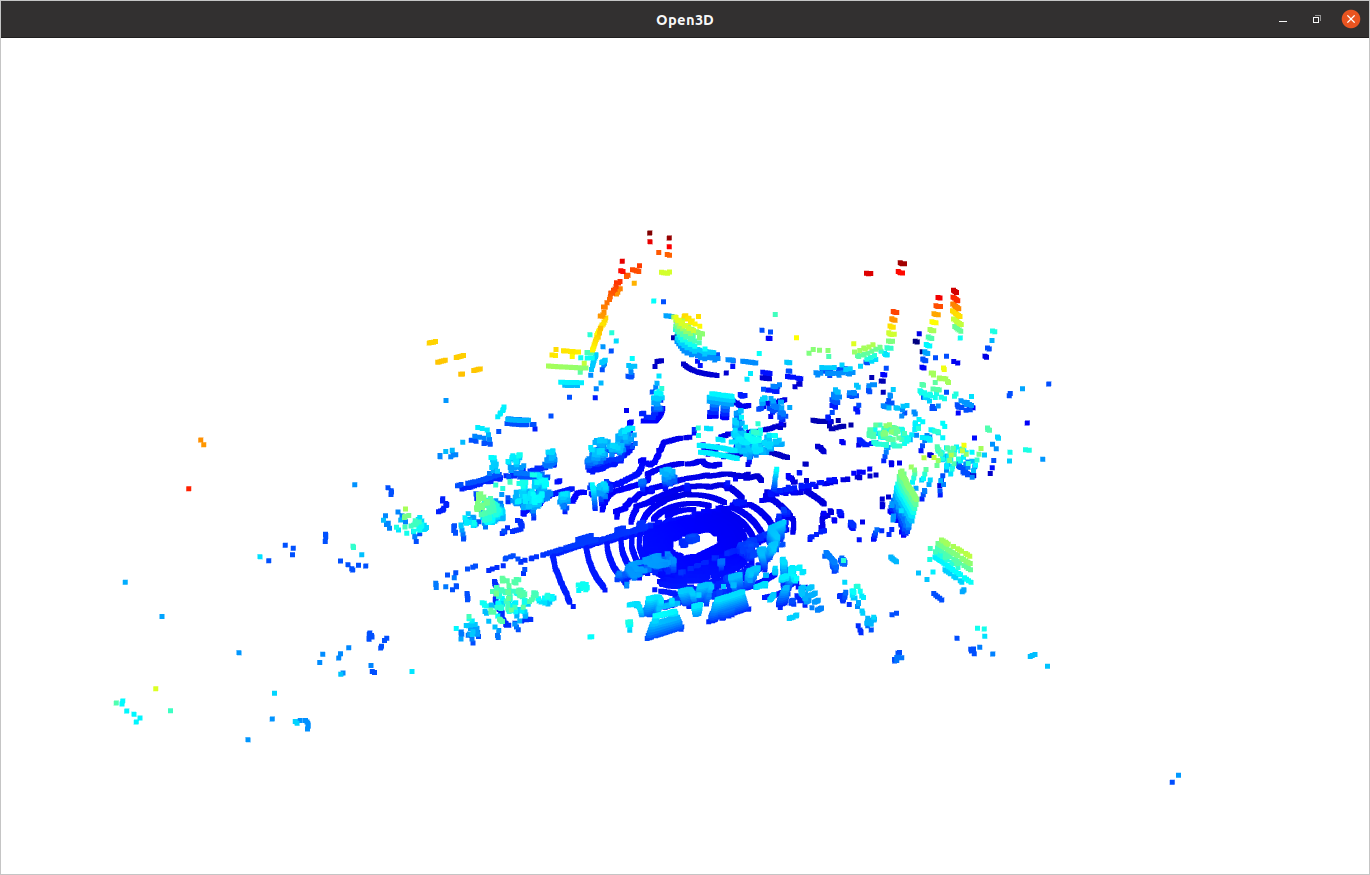
\includegraphics[width=6cm]{fig1a.png}
		\subcaption{Initial pointcloud}
	\end{minipage}
	\begin{minipage}[t]{0.4\textwidth}
		\centering
		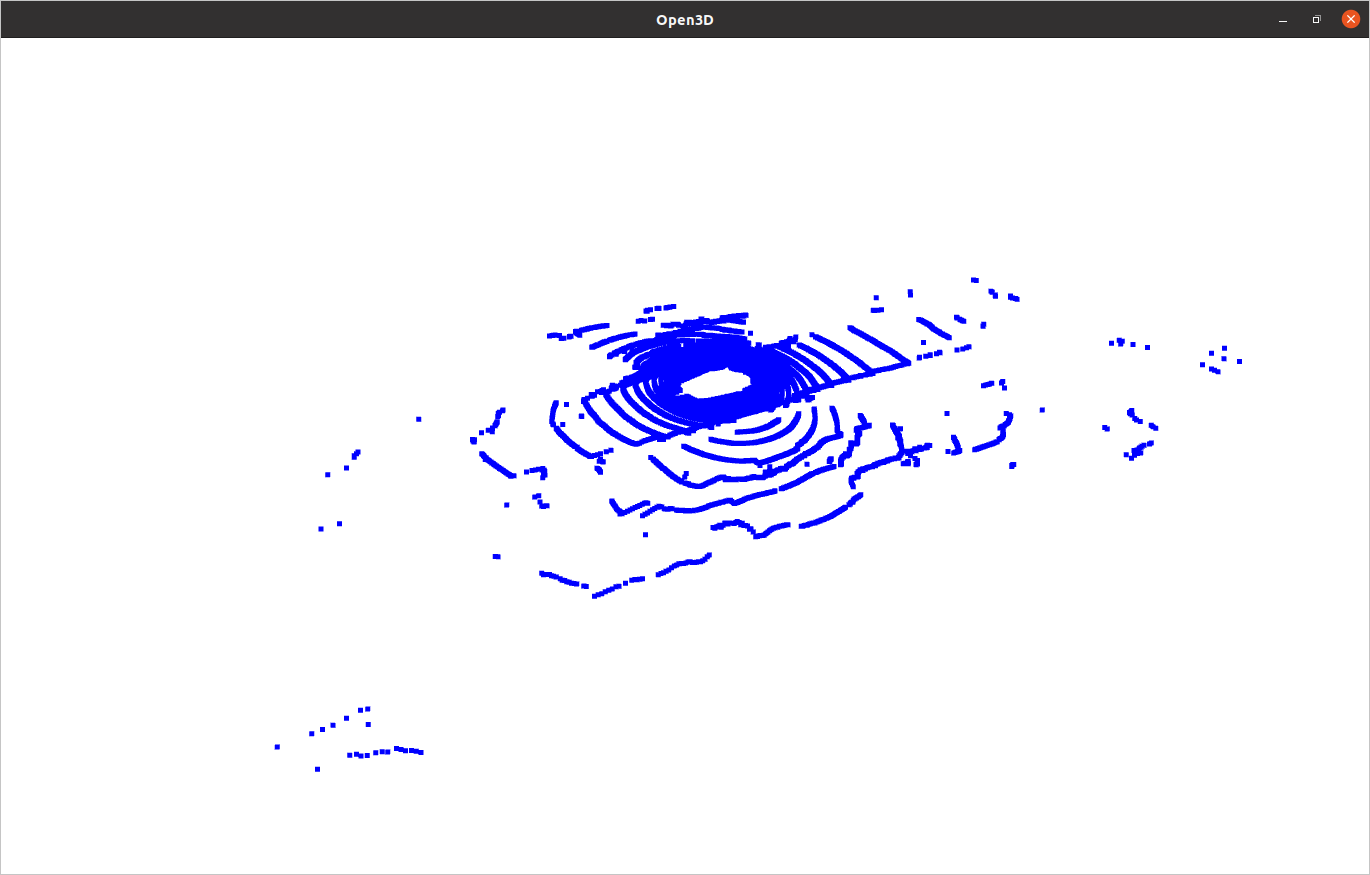
\includegraphics[width=6cm]{fig1b.png}
		\subcaption{Segmented ground pointcloud}
	\end{minipage}
	\caption{Cloud points before and after ground segmentaion in frame1}
	\label{fig1}
\end{figure} 



\subsection{DBSCAN Algorithm}

\hspace{1.0em}
DBSCAN (Density-Based Spatial Clustering of Applications with Noise) algorithm clusters the objects based on density. It defines a cluster as the maximal set of density-reachable points and is able to detect clusters of any shape. DBSCAN has only two parameters $eps$ and $min\_samples$, which defines the core samples that are in areas of high density. As shown in Fig.~\ref{fig2}, the red points are core samples since there are more than $min\_samples$ (5) points around them in $eps$ distance. Those density-reachable core samples and non-core samples (black ones) around them forms a cluster. Therefore, there are 2 clusters in Fig.~\ref{fig2}, and those black points outside circles are detected as noise points.


\begin{figure}[H]
	\centering
	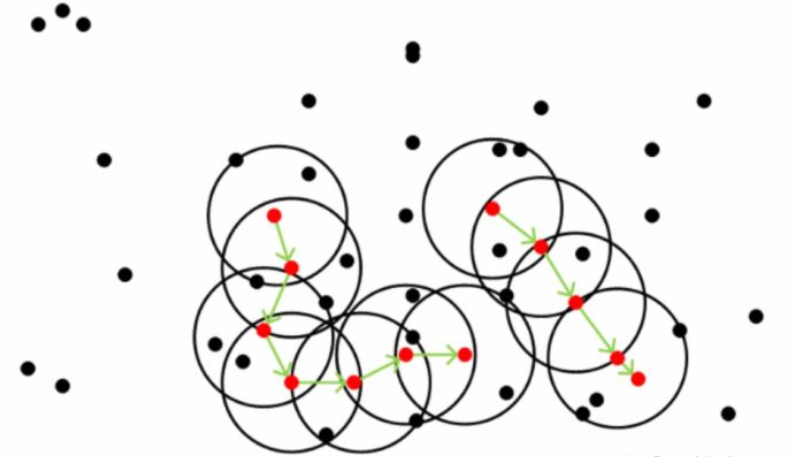
\includegraphics[width=6cm]{fig2.png}
	\caption{DBSCAN clustering principle}
	\label{fig2}
\end{figure} 

We paint the segmented ground point cloud blue and don't use them for clustering. We label different clusters in the scene with different colors, and mark noise points white. Since there may be large number of clusters, the colors of different clusters can be close, we plot bounding boxes for each cluster and store their information in the json file. We test the DBSCAN algorithm with different $eps$ and $min\_samples$, the results are shown in Fig.~\ref{fig3}.

\begin{figure}[H]
	\centering
	\begin{minipage}[t]{0.4\textwidth}
		\centering
		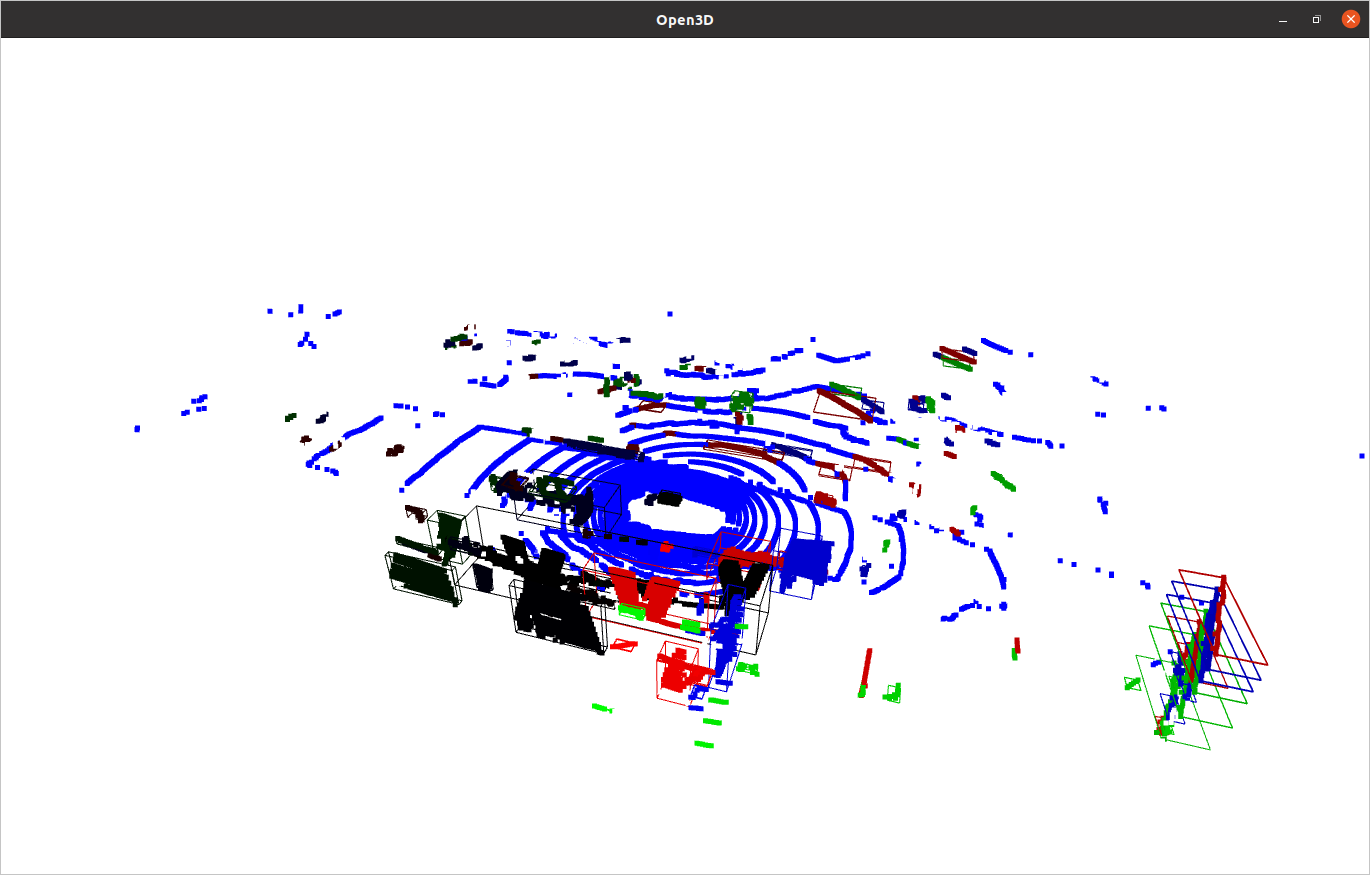
\includegraphics[width=6cm]{fig3a.png}
		\subcaption{$eps=0.5$, $min\_samples=5$ \\ \centering $n\_cluster=166$, $n\_noise=3256$}
		\label{fig3a}
	\end{minipage}
	\begin{minipage}[t]{0.4\textwidth}
		\centering
		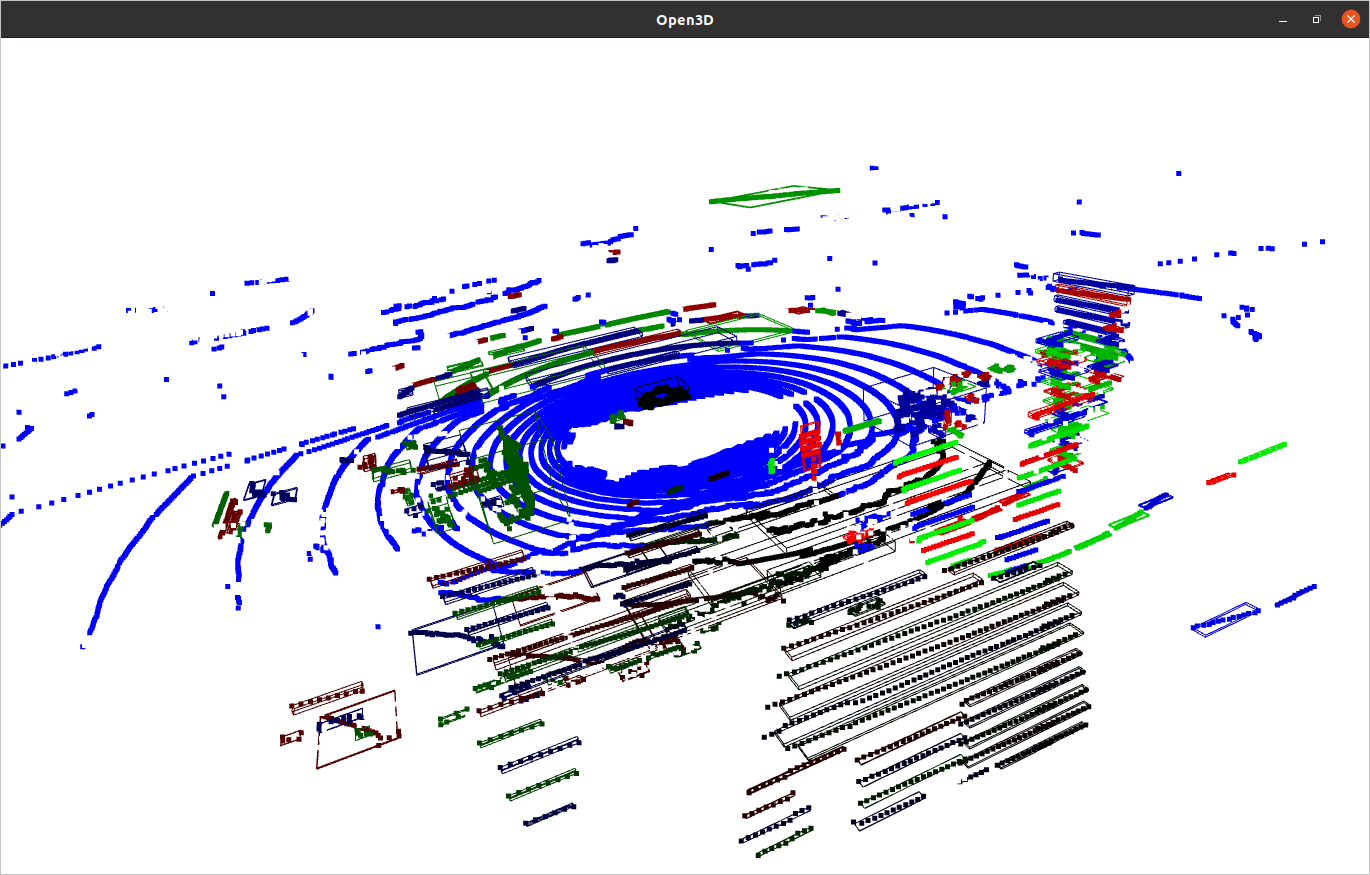
\includegraphics[width=6cm]{fig3b.png}
		\subcaption{$eps=0.25$, $min\_samples=5$ \\ \centering $n\_cluster=200$, $n\_noise=5835$}
		\label{fig3b}
	\end{minipage}
	\begin{minipage}[t]{0.4\textwidth}
		\centering
		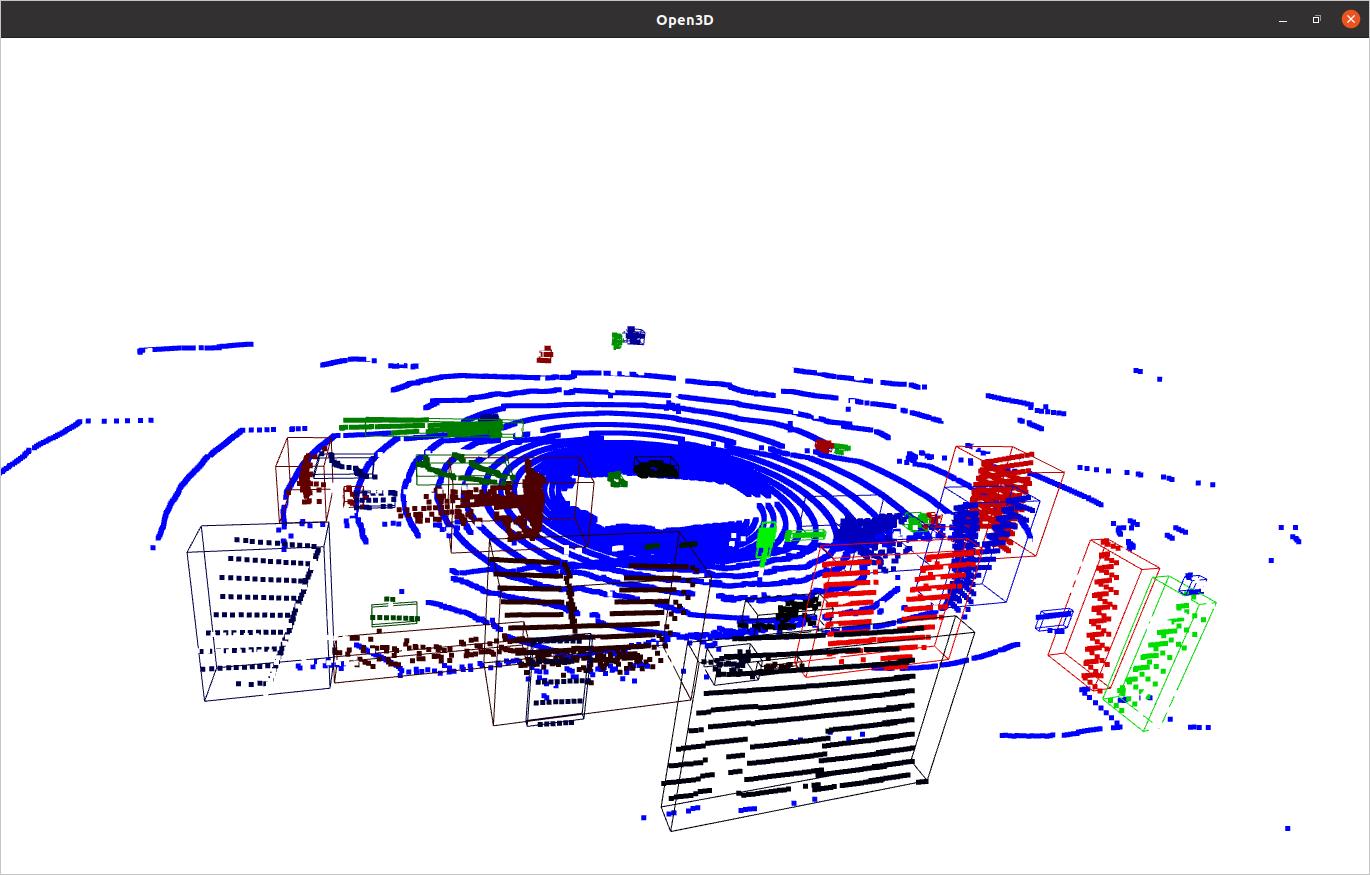
\includegraphics[width=6cm]{fig3c.png}
		\subcaption{$eps=0.5$, $min\_samples=10$ \\ \centering $n\_cluster=44$, $n\_noise=4847$}
		\label{fig3c}
	\end{minipage}
	\begin{minipage}[t]{0.4\textwidth}
		\centering
		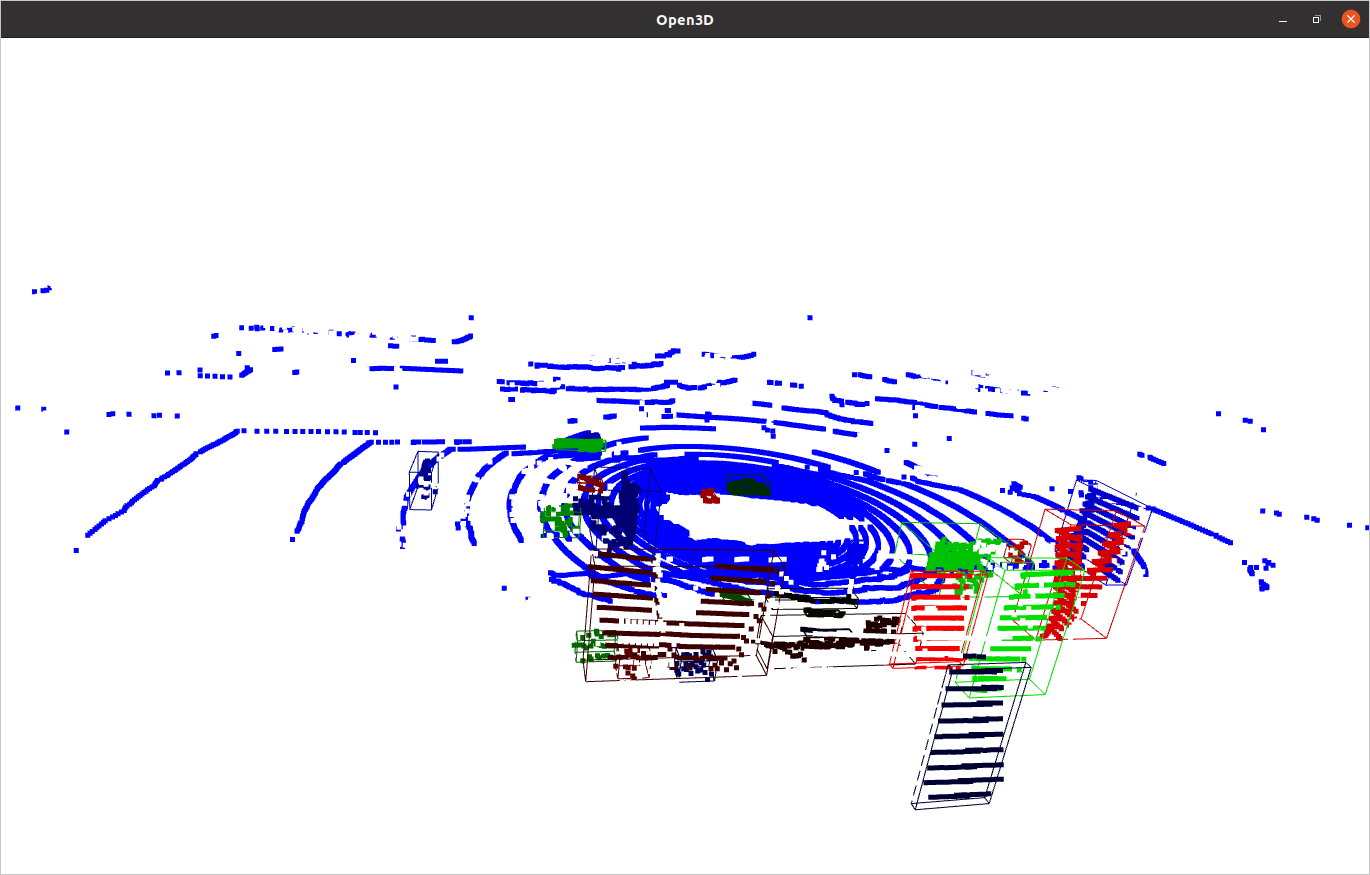
\includegraphics[width=6cm]{fig3d.png}
		\subcaption{$eps=0.5$, $min\_samples=20$ \\ \centering $n\_cluster=21$, $n\_noise=6750$}
		\label{fig3d}
	\end{minipage}
	\caption{Clustering results by DBSCAN algorithm for frame1}
	\label{fig3}
\end{figure} 

It is easy to see that larger $min\_samples$ or smaller $eps$ stands for higher density to form a cluster. In Fig.~\ref{fig3b}, the density requirement is too high and causes bad clustering performance and large number of noise points. Also compare Fig.~\ref{fig3c} and Fig.~\ref{fig3d}, where we remain $eps$ the same and increase the $min\_samples$ requirements, we can find the clustering accuracy increases but it loses more information and generates more noise points. We finally choose the case Fig.~\ref{fig3c} as results written to the json file.

\subsection{Comparison between Different Clustering Methods}

\hspace{1.0em}
OPTICS is an extension version of DBSCAN and make the algorithm no longer sensitive to the radius $eps$. Given the $min\_samples$, OPTICS algorithm will produce an augmented cluster order for analysis and automatically choose the appropriate $eps$. Here we remain $min\_samples=10$ and the result is shown in Fig.~\ref{fig4a}, where more clusters are formed but some noise is also included.

Meanshift is another density-based clustering algorithm. It assumes that different clusters conform to different probability density distributions and aims at finding the fastest direction in which the sample density increases. The areas with high density correspond to the maximum value of the distribution, so data points should belong to one cluster if their density converge to the local maximum. Meanshift adjusts number of clusters by bandwidth, and here we set $quantile=0.01, n\_samples=1000$ to estimate the bandwidth, the result is shown in Fig.~\ref{fig4b} 

Birch algorithm builds an Clustering Feature Tree to realize quick clustering. It is computationally efficient and suits for large dataset. Usually Birch needs some priori knowledge about cluster number and cannot directly detect noise points, which requires removing some mini-cluster afterwards. The results is shown in Fig.~\ref{fig4c} where we set estimated cluster number to be 100. The results of CF Tree can be optimized by hierarchical clustering methods such as AgglomerativeClustering (Fig.~\ref{fig4d}, $n\_clusters=100$). 

K-Means is a partition-based clustering algorithm that uses distance as a measure of similarity between data objects. We also set $n\_clusters=100$ and $tol=0.001$, the results is shown in Fig.~\ref{fig4e}.

\begin{figure}[H]
	\centering
	\begin{minipage}[t]{0.3\textwidth}
		\centering
		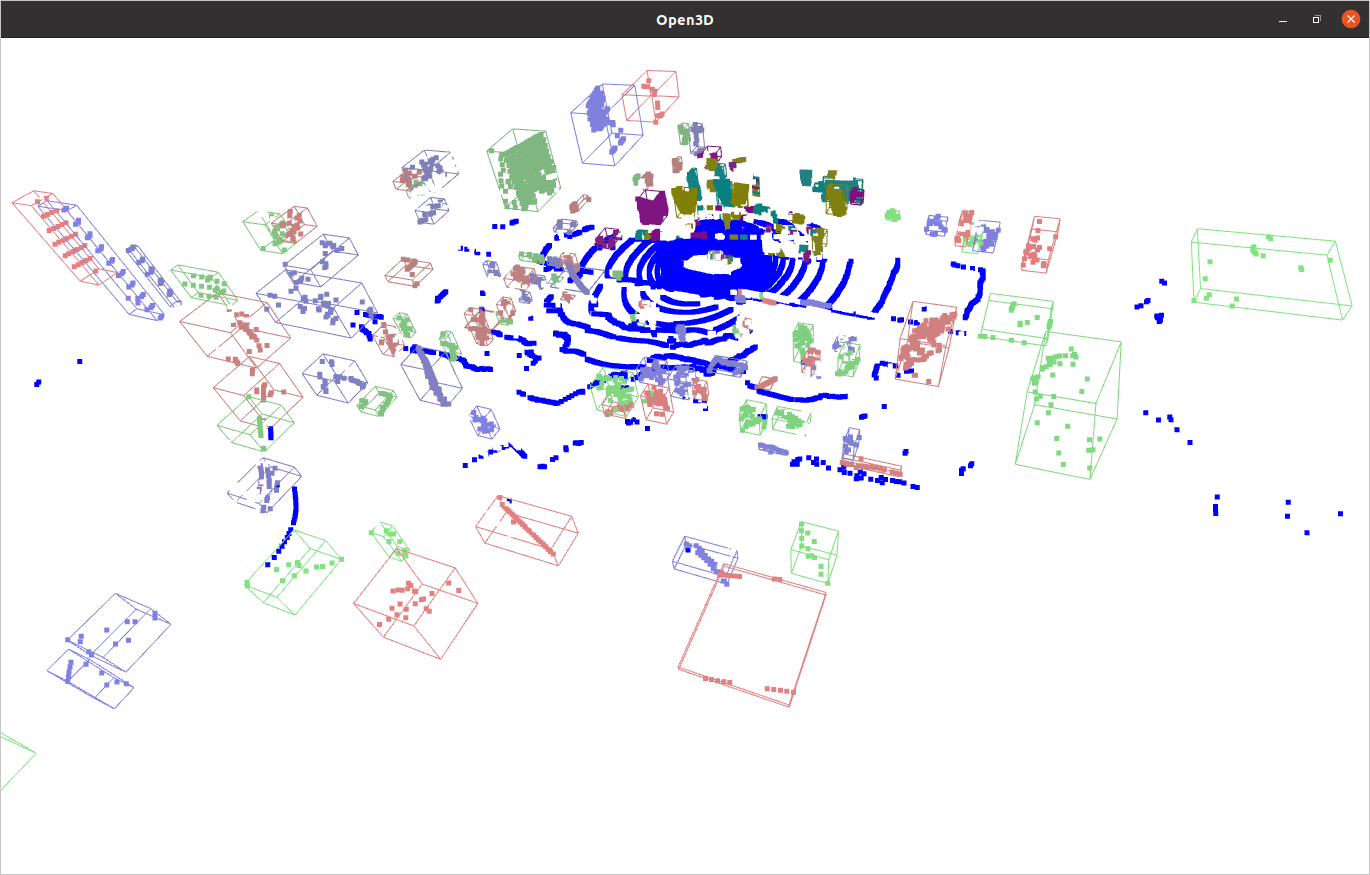
\includegraphics[width=4cm]{fig4a.png}
		\subcaption{OPTICS}
		%  \\ \centering $n\_cluster=432$, $n\_noise=7080$
		\label{fig4a}
	\end{minipage}
	\begin{minipage}[t]{0.3\textwidth}
		\centering
		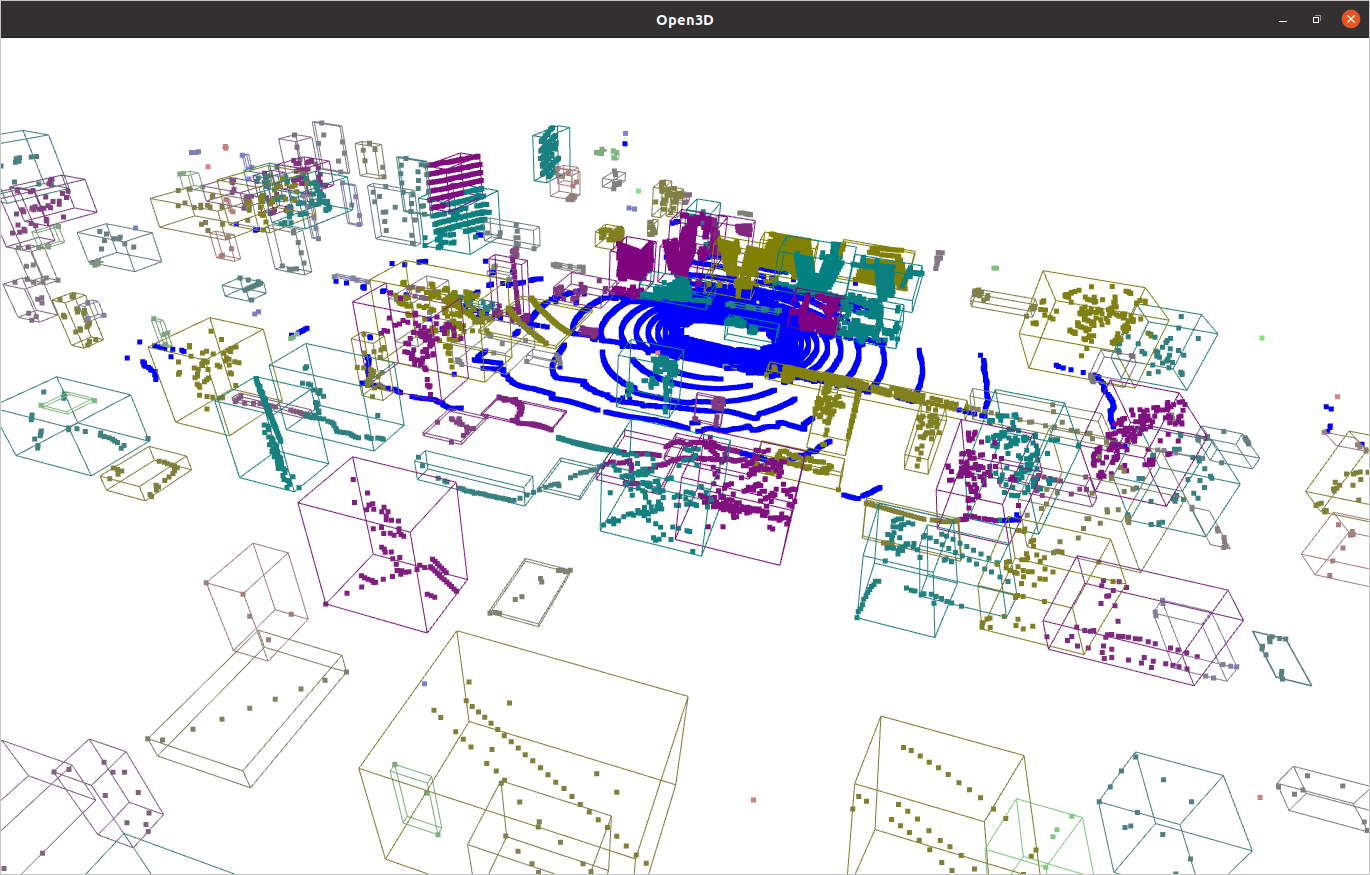
\includegraphics[width=4cm]{fig4e.png}
		\subcaption{Mean Shift}
		\label{fig4b}
	\end{minipage}
	\begin{minipage}[t]{0.3\textwidth}
		\centering
		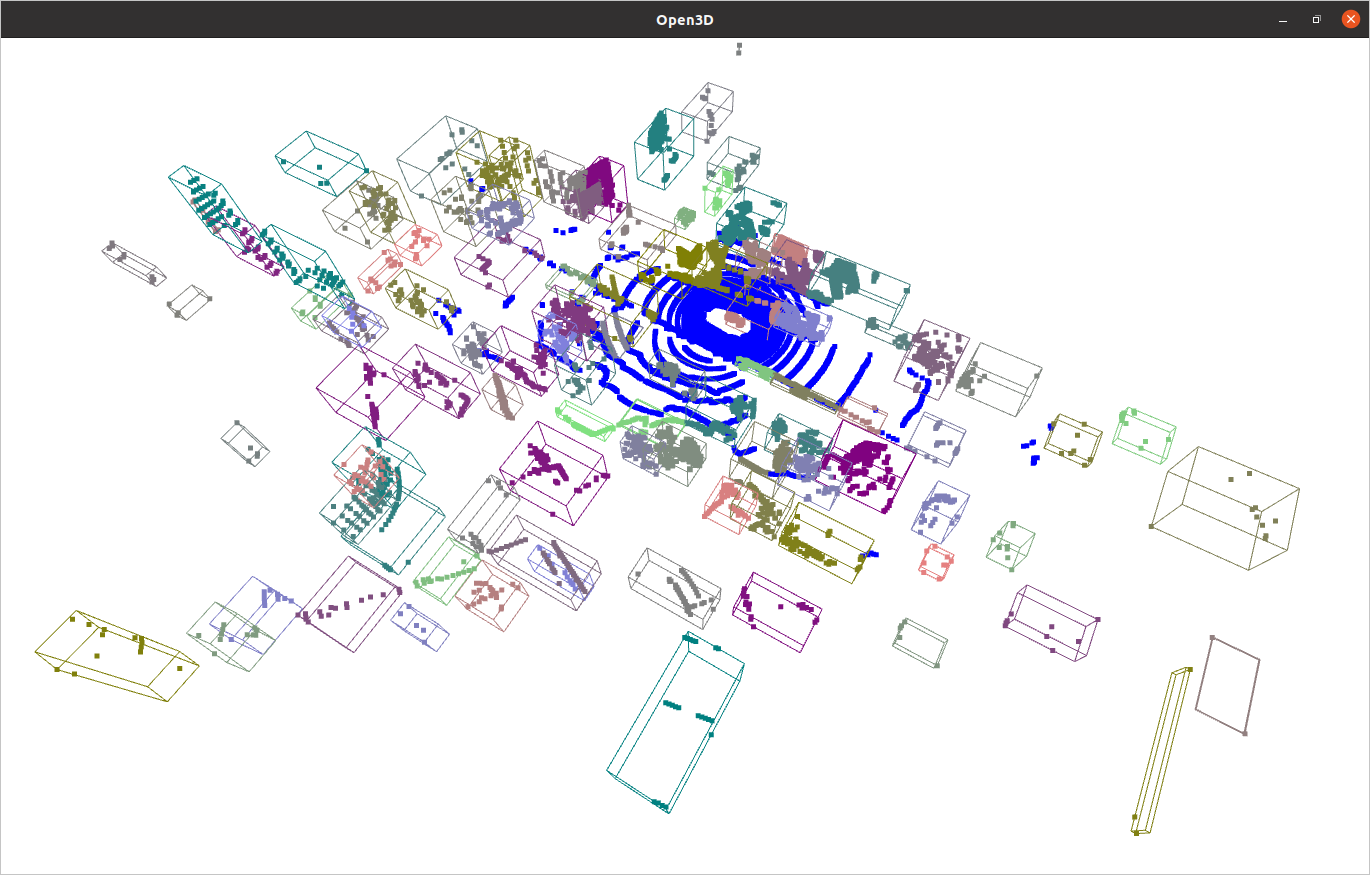
\includegraphics[width=4cm]{fig4b.png}
		\subcaption{Birch}
		\label{fig4c}
	\end{minipage}
	\begin{minipage}[t]{0.3\textwidth}
		\centering
		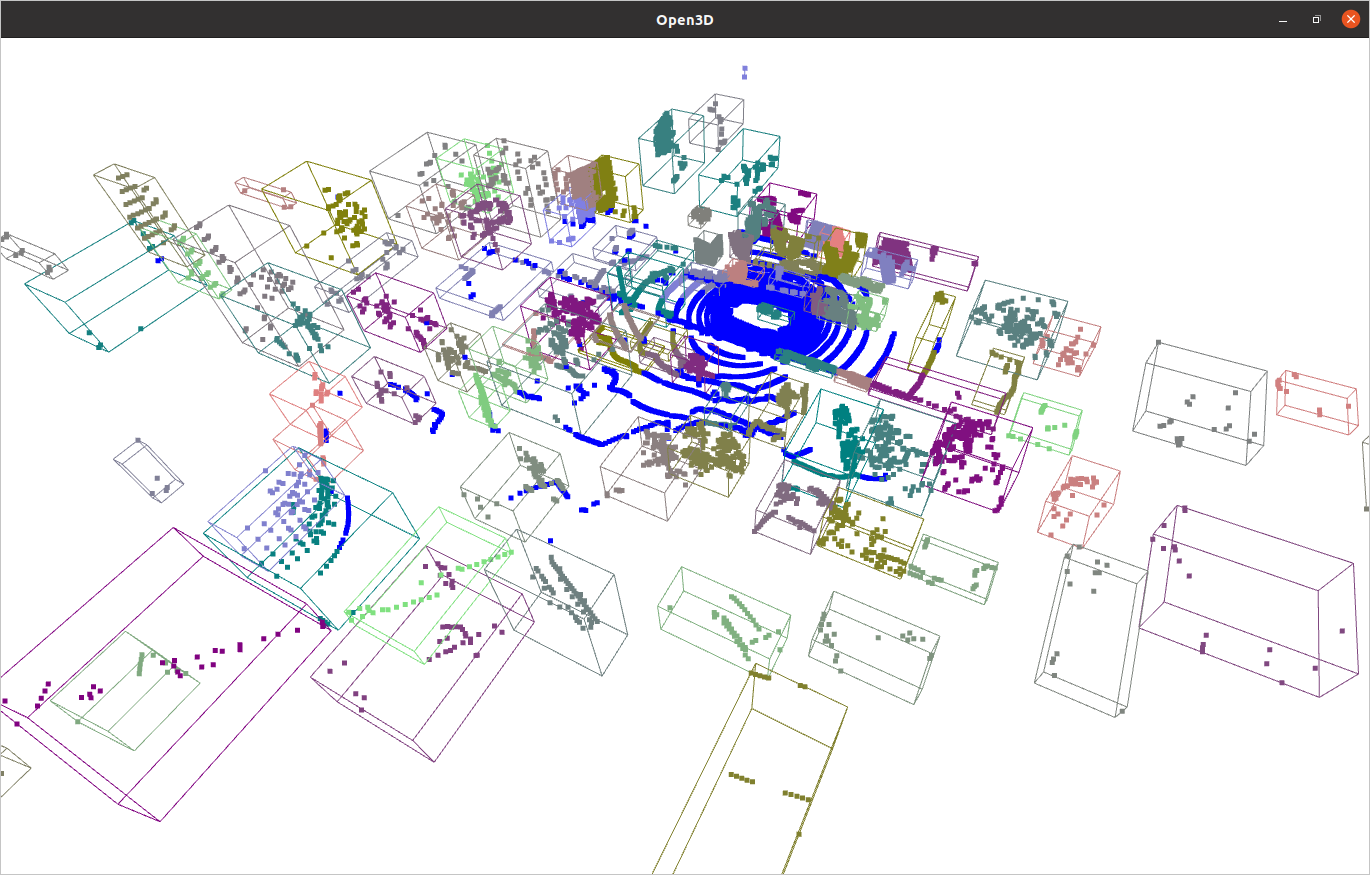
\includegraphics[width=4cm]{fig4c.png}
		\subcaption{Agglomerative Cluster}
		\label{fig4d}
	\end{minipage}
	\begin{minipage}[t]{0.3\textwidth}
		\centering
		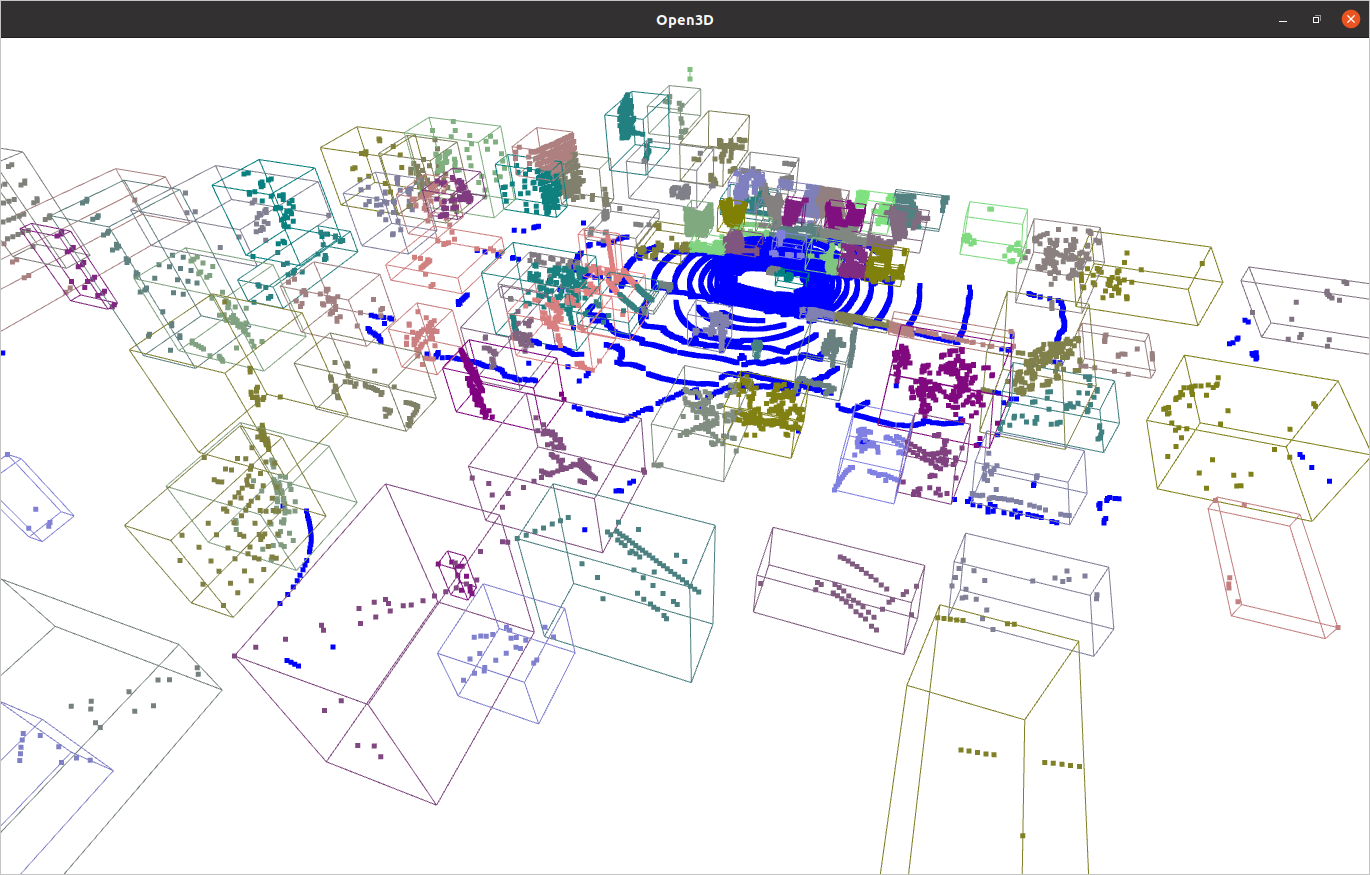
\includegraphics[width=4cm]{fig4d.png}
		\subcaption{KMeans}
		\label{fig4e}
	\end{minipage}
	\begin{minipage}[t]{0.3\textwidth}
		\centering
		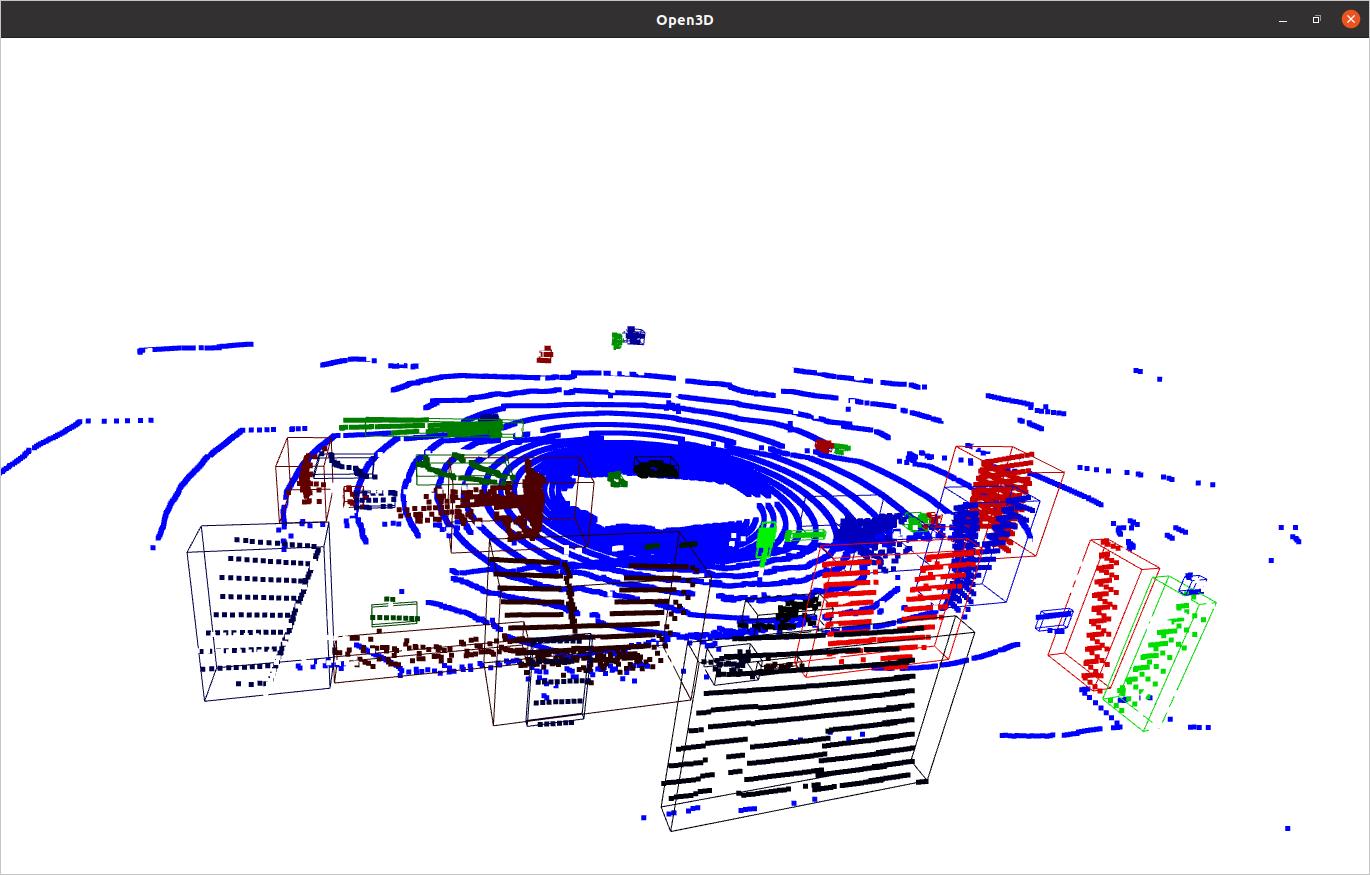
\includegraphics[width=4cm]{fig3c.png}
		\subcaption{DBSCAN}
		\label{fig4f}
	\end{minipage}
	\caption{Comparison between different clustering algorithm for frame1}
	\label{fig4}
\end{figure} 


From the experiment results, we find that Birch, AgglomerativeCluster and KMeans need prior knowledge of cluster numbers and are easy to include noise points. Among them, K-Means can only process convex clustering. Density-based methods instead can do clustering without estimating the total number of clusters, and DBSCAN \& OPTICS perform well in our scenes. 











	
\end{document}








